% Options for packages loaded elsewhere
\PassOptionsToPackage{unicode}{hyperref}
\PassOptionsToPackage{hyphens}{url}
\PassOptionsToPackage{dvipsnames,svgnames,x11names}{xcolor}
%
\documentclass[
  letterpaper,
  DIV=11,
  numbers=noendperiod]{scrartcl}

\usepackage{amsmath,amssymb}
\usepackage{iftex}
\ifPDFTeX
  \usepackage[T1]{fontenc}
  \usepackage[utf8]{inputenc}
  \usepackage{textcomp} % provide euro and other symbols
\else % if luatex or xetex
  \usepackage{unicode-math}
  \defaultfontfeatures{Scale=MatchLowercase}
  \defaultfontfeatures[\rmfamily]{Ligatures=TeX,Scale=1}
\fi
\usepackage{lmodern}
\ifPDFTeX\else  
    % xetex/luatex font selection
\fi
% Use upquote if available, for straight quotes in verbatim environments
\IfFileExists{upquote.sty}{\usepackage{upquote}}{}
\IfFileExists{microtype.sty}{% use microtype if available
  \usepackage[]{microtype}
  \UseMicrotypeSet[protrusion]{basicmath} % disable protrusion for tt fonts
}{}
\makeatletter
\@ifundefined{KOMAClassName}{% if non-KOMA class
  \IfFileExists{parskip.sty}{%
    \usepackage{parskip}
  }{% else
    \setlength{\parindent}{0pt}
    \setlength{\parskip}{6pt plus 2pt minus 1pt}}
}{% if KOMA class
  \KOMAoptions{parskip=half}}
\makeatother
\usepackage{xcolor}
\setlength{\emergencystretch}{3em} % prevent overfull lines
\setcounter{secnumdepth}{-\maxdimen} % remove section numbering
% Make \paragraph and \subparagraph free-standing
\makeatletter
\ifx\paragraph\undefined\else
  \let\oldparagraph\paragraph
  \renewcommand{\paragraph}{
    \@ifstar
      \xxxParagraphStar
      \xxxParagraphNoStar
  }
  \newcommand{\xxxParagraphStar}[1]{\oldparagraph*{#1}\mbox{}}
  \newcommand{\xxxParagraphNoStar}[1]{\oldparagraph{#1}\mbox{}}
\fi
\ifx\subparagraph\undefined\else
  \let\oldsubparagraph\subparagraph
  \renewcommand{\subparagraph}{
    \@ifstar
      \xxxSubParagraphStar
      \xxxSubParagraphNoStar
  }
  \newcommand{\xxxSubParagraphStar}[1]{\oldsubparagraph*{#1}\mbox{}}
  \newcommand{\xxxSubParagraphNoStar}[1]{\oldsubparagraph{#1}\mbox{}}
\fi
\makeatother

\usepackage{color}
\usepackage{fancyvrb}
\newcommand{\VerbBar}{|}
\newcommand{\VERB}{\Verb[commandchars=\\\{\}]}
\DefineVerbatimEnvironment{Highlighting}{Verbatim}{commandchars=\\\{\}}
% Add ',fontsize=\small' for more characters per line
\usepackage{framed}
\definecolor{shadecolor}{RGB}{241,243,245}
\newenvironment{Shaded}{\begin{snugshade}}{\end{snugshade}}
\newcommand{\AlertTok}[1]{\textcolor[rgb]{0.68,0.00,0.00}{#1}}
\newcommand{\AnnotationTok}[1]{\textcolor[rgb]{0.37,0.37,0.37}{#1}}
\newcommand{\AttributeTok}[1]{\textcolor[rgb]{0.40,0.45,0.13}{#1}}
\newcommand{\BaseNTok}[1]{\textcolor[rgb]{0.68,0.00,0.00}{#1}}
\newcommand{\BuiltInTok}[1]{\textcolor[rgb]{0.00,0.23,0.31}{#1}}
\newcommand{\CharTok}[1]{\textcolor[rgb]{0.13,0.47,0.30}{#1}}
\newcommand{\CommentTok}[1]{\textcolor[rgb]{0.37,0.37,0.37}{#1}}
\newcommand{\CommentVarTok}[1]{\textcolor[rgb]{0.37,0.37,0.37}{\textit{#1}}}
\newcommand{\ConstantTok}[1]{\textcolor[rgb]{0.56,0.35,0.01}{#1}}
\newcommand{\ControlFlowTok}[1]{\textcolor[rgb]{0.00,0.23,0.31}{\textbf{#1}}}
\newcommand{\DataTypeTok}[1]{\textcolor[rgb]{0.68,0.00,0.00}{#1}}
\newcommand{\DecValTok}[1]{\textcolor[rgb]{0.68,0.00,0.00}{#1}}
\newcommand{\DocumentationTok}[1]{\textcolor[rgb]{0.37,0.37,0.37}{\textit{#1}}}
\newcommand{\ErrorTok}[1]{\textcolor[rgb]{0.68,0.00,0.00}{#1}}
\newcommand{\ExtensionTok}[1]{\textcolor[rgb]{0.00,0.23,0.31}{#1}}
\newcommand{\FloatTok}[1]{\textcolor[rgb]{0.68,0.00,0.00}{#1}}
\newcommand{\FunctionTok}[1]{\textcolor[rgb]{0.28,0.35,0.67}{#1}}
\newcommand{\ImportTok}[1]{\textcolor[rgb]{0.00,0.46,0.62}{#1}}
\newcommand{\InformationTok}[1]{\textcolor[rgb]{0.37,0.37,0.37}{#1}}
\newcommand{\KeywordTok}[1]{\textcolor[rgb]{0.00,0.23,0.31}{\textbf{#1}}}
\newcommand{\NormalTok}[1]{\textcolor[rgb]{0.00,0.23,0.31}{#1}}
\newcommand{\OperatorTok}[1]{\textcolor[rgb]{0.37,0.37,0.37}{#1}}
\newcommand{\OtherTok}[1]{\textcolor[rgb]{0.00,0.23,0.31}{#1}}
\newcommand{\PreprocessorTok}[1]{\textcolor[rgb]{0.68,0.00,0.00}{#1}}
\newcommand{\RegionMarkerTok}[1]{\textcolor[rgb]{0.00,0.23,0.31}{#1}}
\newcommand{\SpecialCharTok}[1]{\textcolor[rgb]{0.37,0.37,0.37}{#1}}
\newcommand{\SpecialStringTok}[1]{\textcolor[rgb]{0.13,0.47,0.30}{#1}}
\newcommand{\StringTok}[1]{\textcolor[rgb]{0.13,0.47,0.30}{#1}}
\newcommand{\VariableTok}[1]{\textcolor[rgb]{0.07,0.07,0.07}{#1}}
\newcommand{\VerbatimStringTok}[1]{\textcolor[rgb]{0.13,0.47,0.30}{#1}}
\newcommand{\WarningTok}[1]{\textcolor[rgb]{0.37,0.37,0.37}{\textit{#1}}}

\providecommand{\tightlist}{%
  \setlength{\itemsep}{0pt}\setlength{\parskip}{0pt}}\usepackage{longtable,booktabs,array}
\usepackage{calc} % for calculating minipage widths
% Correct order of tables after \paragraph or \subparagraph
\usepackage{etoolbox}
\makeatletter
\patchcmd\longtable{\par}{\if@noskipsec\mbox{}\fi\par}{}{}
\makeatother
% Allow footnotes in longtable head/foot
\IfFileExists{footnotehyper.sty}{\usepackage{footnotehyper}}{\usepackage{footnote}}
\makesavenoteenv{longtable}
\usepackage{graphicx}
\makeatletter
\def\maxwidth{\ifdim\Gin@nat@width>\linewidth\linewidth\else\Gin@nat@width\fi}
\def\maxheight{\ifdim\Gin@nat@height>\textheight\textheight\else\Gin@nat@height\fi}
\makeatother
% Scale images if necessary, so that they will not overflow the page
% margins by default, and it is still possible to overwrite the defaults
% using explicit options in \includegraphics[width, height, ...]{}
\setkeys{Gin}{width=\maxwidth,height=\maxheight,keepaspectratio}
% Set default figure placement to htbp
\makeatletter
\def\fps@figure{htbp}
\makeatother

\usepackage{booktabs}
\usepackage{longtable}
\usepackage{array}
\usepackage{multirow}
\usepackage{wrapfig}
\usepackage{float}
\usepackage{colortbl}
\usepackage{pdflscape}
\usepackage{tabu}
\usepackage{threeparttable}
\usepackage{threeparttablex}
\usepackage[normalem]{ulem}
\usepackage{makecell}
\usepackage{xcolor}
\KOMAoption{captions}{tableheading}
\makeatletter
\@ifpackageloaded{caption}{}{\usepackage{caption}}
\AtBeginDocument{%
\ifdefined\contentsname
  \renewcommand*\contentsname{Table of contents}
\else
  \newcommand\contentsname{Table of contents}
\fi
\ifdefined\listfigurename
  \renewcommand*\listfigurename{List of Figures}
\else
  \newcommand\listfigurename{List of Figures}
\fi
\ifdefined\listtablename
  \renewcommand*\listtablename{List of Tables}
\else
  \newcommand\listtablename{List of Tables}
\fi
\ifdefined\figurename
  \renewcommand*\figurename{Figure}
\else
  \newcommand\figurename{Figure}
\fi
\ifdefined\tablename
  \renewcommand*\tablename{Table}
\else
  \newcommand\tablename{Table}
\fi
}
\@ifpackageloaded{float}{}{\usepackage{float}}
\floatstyle{ruled}
\@ifundefined{c@chapter}{\newfloat{codelisting}{h}{lop}}{\newfloat{codelisting}{h}{lop}[chapter]}
\floatname{codelisting}{Listing}
\newcommand*\listoflistings{\listof{codelisting}{List of Listings}}
\makeatother
\makeatletter
\makeatother
\makeatletter
\@ifpackageloaded{caption}{}{\usepackage{caption}}
\@ifpackageloaded{subcaption}{}{\usepackage{subcaption}}
\makeatother

\ifLuaTeX
  \usepackage{selnolig}  % disable illegal ligatures
\fi
\usepackage{bookmark}

\IfFileExists{xurl.sty}{\usepackage{xurl}}{} % add URL line breaks if available
\urlstyle{same} % disable monospaced font for URLs
\hypersetup{
  pdftitle={Mini Project \#4},
  pdfauthor={Gwynnie Hayes},
  colorlinks=true,
  linkcolor={blue},
  filecolor={Maroon},
  citecolor={Blue},
  urlcolor={Blue},
  pdfcreator={LaTeX via pandoc}}


\title{Mini Project \#4}
\usepackage{etoolbox}
\makeatletter
\providecommand{\subtitle}[1]{% add subtitle to \maketitle
  \apptocmd{\@title}{\par {\large #1 \par}}{}{}
}
\makeatother
\subtitle{Text Analysis}
\author{Gwynnie Hayes}
\date{}

\begin{document}
\maketitle


\section{Introduction}\label{introduction}

One of my favorite bands is called Illuminati Hotties, what I love about
them is that all the songs are very different and unique. The main
artist is named Sarah Tudzin and in her professional life she is a music
producer for many much more popular artists. She also writes and
produces her own music and what I think is really cool about it is she
just has fun making a bunch of cool and unique sounds, that aren't
dictated by someone else.

Some of my friends and I went to a concert for another artist called Pom
Pom Squad almost 6 years ago at this point where we were first
introduced to her and have been hooked ever since, one of the things we
always talk about is the uniqueness of her music and the interesting and
sometimes slightly disturbing lyrics she uses in her songs. This led me
to wanting to do a text analysis of her song lyrics.

\section{Data!}\label{data}

There was not a data set of her song lyrics as she is not a very famous
artist so i made the maybe silly decision to scrape all the lyrics off
the web myself and make my own data set. I did all of this in a document
called MP4\_cleaning.qmd because it was a lot of code that was not
important to the actual project results, it is however linked in my
github and on this website page.

What I did was used the web page scraping functions that we made in
class to make a similar function that I could input the names of the
songs into. I first tried to do all the songs at once but was running
into issues with my IP address getting blocked from requesting too much
data so I had to break down the songs into smaller requests and I made
10 individual csv files that I then bind\_row() into one full data set.
This however was only the names of the songs and the lyrics and I wanted
an album name which was a little more complicated because the website I
used to get the lyrics did not have the album name on the page that the
song lyrics were on. So I just did a bunch of if else statements to add
the new column. This definitely was not the most efficient method of
doing this but its what I did because it was more familiar for a part of
the project that was completely unnecessary.

\begin{longtable}[]{@{}lll@{}}
\toprule\noalign{}
Song & word & album \\
\midrule\noalign{}
\endhead
\bottomrule\noalign{}
\endlastfoot
(You're Better) Than Ever & all & Kiss Yr Frenemies \\
(You're Better) Than Ever & my & Kiss Yr Frenemies \\
(You're Better) Than Ever & favorite & Kiss Yr Frenemies \\
(You're Better) Than Ever & socks & Kiss Yr Frenemies \\
(You're Better) Than Ever & are & Kiss Yr Frenemies \\
(You're Better) Than Ever & getting & Kiss Yr Frenemies \\
\end{longtable}

This is what the data set looks like after I read it into this document
and did some final cleaning!

Illuminati Hotties have 5 albums and a couple singles that I am
analyzing together as one ``album''.

\begin{figure}[H]

{\centering 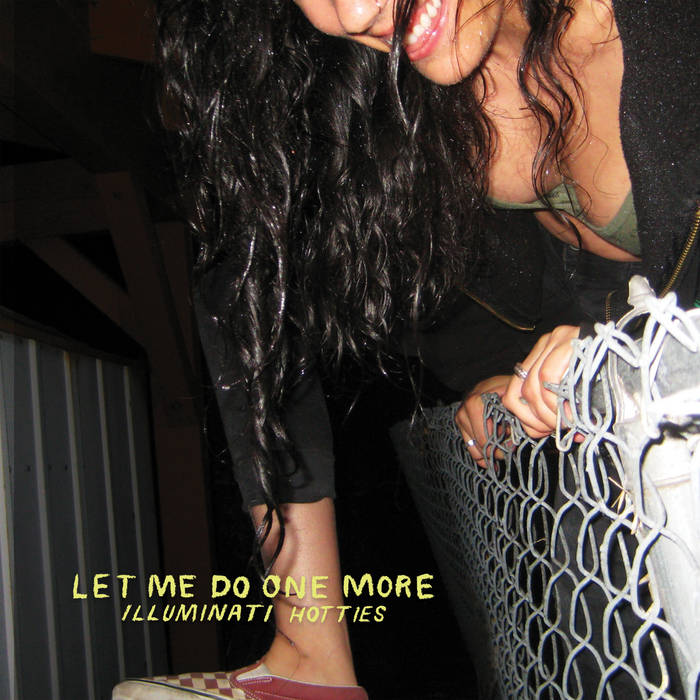
\includegraphics{media/letmedoonemoe.jpg}

}

\caption{Let Me Do One More}

\end{figure}%

\begin{figure}[H]

{\centering 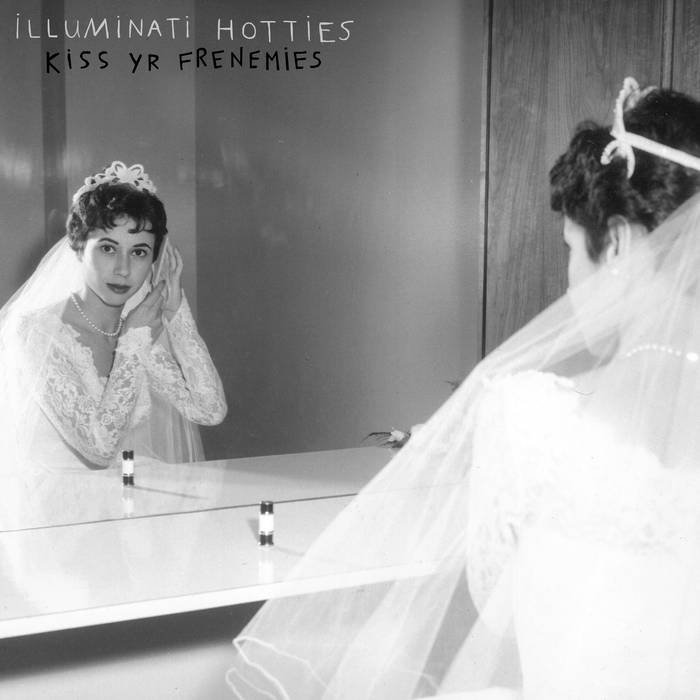
\includegraphics{media/kissyrfrenemies.jpg}

}

\caption{Kiss Yr Frenemies}

\end{figure}%

\begin{figure}[H]

{\centering 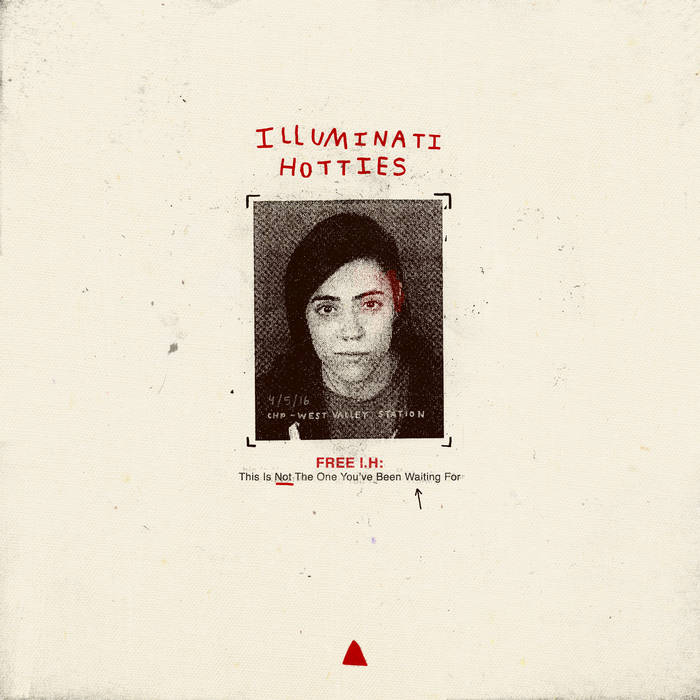
\includegraphics{media/freeih.jpg}

}

\caption{Free I.H: This is Not the One You've Been Waiting For}

\end{figure}%

\begin{figure}[H]

{\centering 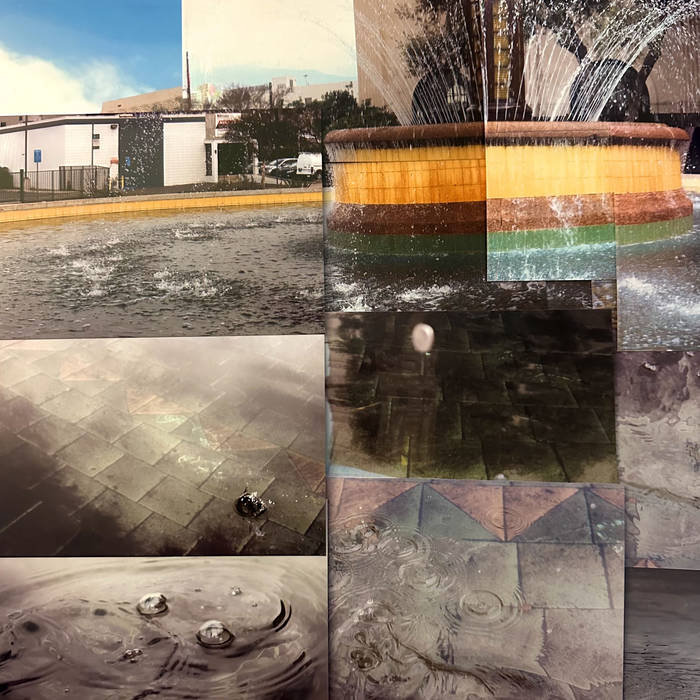
\includegraphics{media/nickelonfountain.jpg}

}

\caption{Nickel on the Fountain Floor}

\end{figure}%

\begin{figure}[H]

{\centering 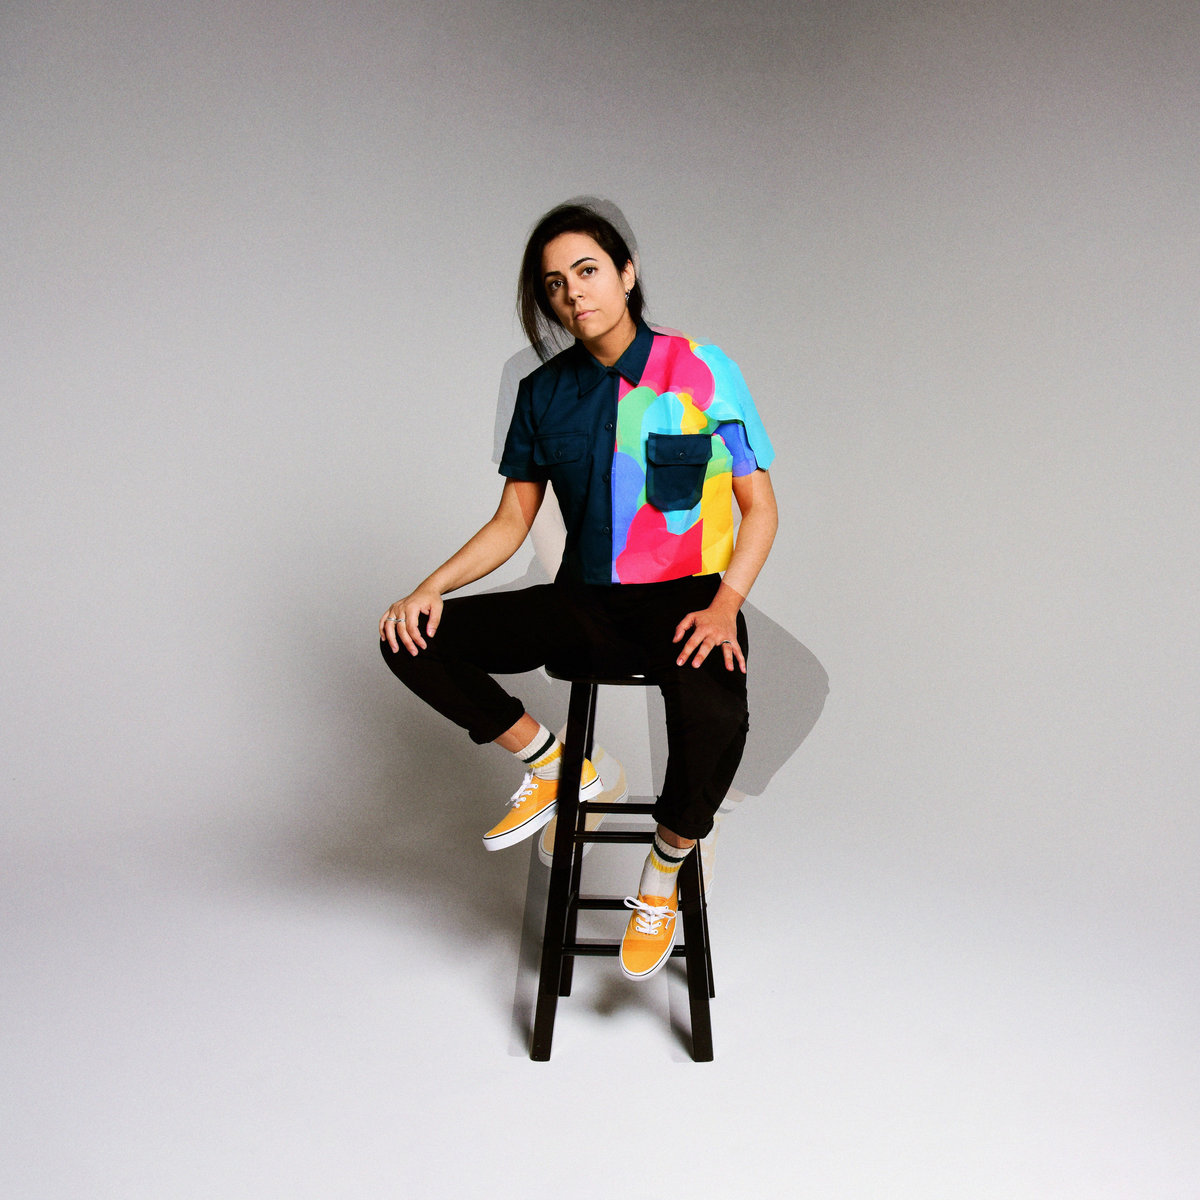
\includegraphics{media/power.jpg}

}

\caption{Power}

\end{figure}%

\section{Questions}\label{questions}

is power more similar to itself then the other albums most common words
most interesting words sentient analysis with out onomatopoeia

\section{Text Analysis}\label{text-analysis}

I first wanted to just look at the most common word in all of her songs
in general:

\begin{longtable}[]{@{}lr@{}}
\toprule\noalign{}
word & n \\
\midrule\noalign{}
\endhead
\bottomrule\noalign{}
\endlastfoot
i & 457 \\
you & 415 \\
the & 300 \\
a & 216 \\
i'm & 178 \\
and & 155 \\
\end{longtable}

I found that the most common word in all of her songs is ``I'' which is
said 457 times.

I then wanted to see the most common word in each of the albums and
found this:

\begin{longtable}[]{@{}llr@{}}
\toprule\noalign{}
album & word & n \\
\midrule\noalign{}
\endhead
\bottomrule\noalign{}
\endlastfoot
FREE I.H: This Is Not the One You've Been Waiting For & you & 59 \\
Kiss Yr Frenemies & i & 100 \\
Nickel on the Fountain Floor & you & 17 \\
Power & i & 121 \\
Single & i & 70 \\
let me do one more & i & 113 \\
\end{longtable}

This includes all of the words, including the most common words I am
more interested in the most used uncommon words. I removed the stop
words using the smart words set of words.

\begin{verbatim}
Joining with `by = join_by(word)`
\end{verbatim}

\begin{longtable}[]{@{}lr@{}}
\toprule\noalign{}
word & n \\
\midrule\noalign{}
\endhead
\bottomrule\noalign{}
\endlastfoot
ah & 111 \\
time & 62 \\
mm & 60 \\
love & 52 \\
wanna & 42 \\
hm & 24 \\
\end{longtable}

\begin{longtable}[]{@{}llr@{}}
\toprule\noalign{}
album & word & n \\
\midrule\noalign{}
\endhead
\bottomrule\noalign{}
\endlastfoot
FREE I.H: This Is Not the One You've Been Waiting For & mm & 36 \\
Kiss Yr Frenemies & time & 15 \\
Nickel on the Fountain Floor & 777 & 7 \\
Power & love & 36 \\
Single & ah & 34 \\
let me do one more & ah & 44 \\
\end{longtable}

Most of these still are not full words and so I should filter them out.

\begin{longtable}[]{@{}lr@{}}
\toprule\noalign{}
word & n \\
\midrule\noalign{}
\endhead
\bottomrule\noalign{}
\endlastfoot
time & 62 \\
love & 52 \\
wanna & 42 \\
play & 21 \\
yeah & 19 \\
bad & 17 \\
\end{longtable}

\begin{longtable}[]{@{}llr@{}}
\toprule\noalign{}
album & word & n \\
\midrule\noalign{}
\endhead
\bottomrule\noalign{}
\endlastfoot
FREE I.H: This Is Not the One You've Been Waiting For & content & 17 \\
Kiss Yr Frenemies & time & 15 \\
Nickel on the Fountain Floor & 777 & 7 \\
Power & love & 36 \\
Single & miss & 11 \\
let me do one more & wanna & 23 \\
\end{longtable}

\begin{verbatim}
# A tibble: 2,477 x 2
   word       value
   <chr>      <dbl>
 1 abandon       -2
 2 abandoned     -2
 3 abandons      -2
 4 abducted      -2
 5 abduction     -2
 6 abductions    -2
 7 abhor         -3
 8 abhorred      -3
 9 abhorrent     -3
10 abhors        -3
# i 2,467 more rows
\end{verbatim}

\begin{verbatim}
# A tibble: 13,872 x 2
   word        sentiment
   <chr>       <chr>    
 1 abacus      trust    
 2 abandon     fear     
 3 abandon     negative 
 4 abandon     sadness  
 5 abandoned   anger    
 6 abandoned   fear     
 7 abandoned   negative 
 8 abandoned   sadness  
 9 abandonment anger    
10 abandonment fear     
# i 13,862 more rows
\end{verbatim}

\begin{verbatim}
# A tibble: 6,786 x 2
   word        sentiment
   <chr>       <chr>    
 1 2-faces     negative 
 2 abnormal    negative 
 3 abolish     negative 
 4 abominable  negative 
 5 abominably  negative 
 6 abominate   negative 
 7 abomination negative 
 8 abort       negative 
 9 aborted     negative 
10 aborts      negative 
# i 6,776 more rows
\end{verbatim}

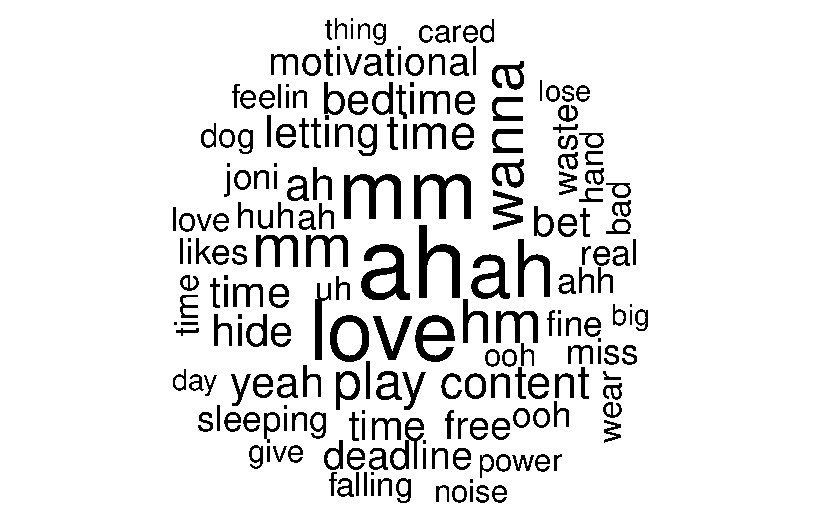
\includegraphics{MP4_files/figure-pdf/unnamed-chunk-9-1.pdf}

\begin{Shaded}
\begin{Highlighting}[]
\NormalTok{snowFreeIH }\SpecialCharTok{|\textgreater{}} 
  \FunctionTok{inner\_join}\NormalTok{(bing\_sentiments) }\SpecialCharTok{|\textgreater{}}
  \FunctionTok{count}\NormalTok{(Song, album, sentiment) }\SpecialCharTok{|\textgreater{}}
  \FunctionTok{pivot\_wider}\NormalTok{(}\AttributeTok{names\_from =}\NormalTok{ sentiment, }\AttributeTok{values\_from =}\NormalTok{ n) }\SpecialCharTok{|\textgreater{}}
  \FunctionTok{mutate}\NormalTok{(}\AttributeTok{sentiment =}\NormalTok{ positive }\SpecialCharTok{{-}}\NormalTok{ negative) }\SpecialCharTok{|\textgreater{}}
  \FunctionTok{ggplot}\NormalTok{(}\FunctionTok{aes}\NormalTok{(}\AttributeTok{x =}\NormalTok{ Song, }\AttributeTok{y =}\NormalTok{ sentiment, }\AttributeTok{fill =}\NormalTok{ album)) }\SpecialCharTok{+}
    \FunctionTok{geom\_col}\NormalTok{(}\AttributeTok{show.legend =} \ConstantTok{FALSE}\NormalTok{) }\SpecialCharTok{+}
  \FunctionTok{theme}\NormalTok{(}\AttributeTok{axis.text.x =} \FunctionTok{element\_text}\NormalTok{(}\AttributeTok{angle =} \DecValTok{75}\NormalTok{, }\AttributeTok{hjust =} \DecValTok{1}\NormalTok{)) }\SpecialCharTok{+}
  \FunctionTok{facet\_grid}\NormalTok{(}\SpecialCharTok{\textasciitilde{}}\NormalTok{album, }\AttributeTok{scales =} \StringTok{"free\_x"}\NormalTok{)}
\end{Highlighting}
\end{Shaded}

\begin{verbatim}
Joining with `by = join_by(word)`
\end{verbatim}

\begin{verbatim}
Warning: Removed 9 rows containing missing values or values outside the scale range
(`geom_col()`).
\end{verbatim}

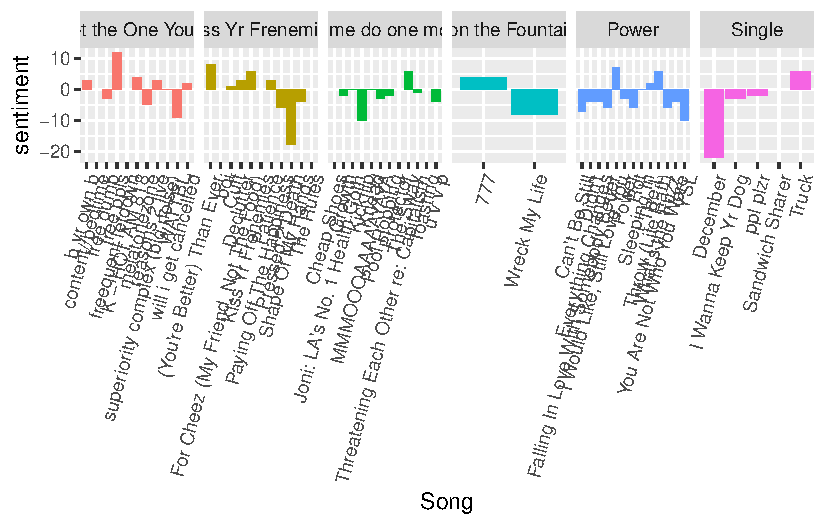
\includegraphics{MP4_files/figure-pdf/unnamed-chunk-10-1.pdf}




\end{document}
